\section{Seweryn Fronc}
\label{sfronc}
\begin{center}
    A black hole (see Figure~\ref{fig:bl}) is a region of spacetime where gravity is so strong that nothing, including light and other electromagnetic waves, has enough energy to escape it.
\end{center}

\begin{figure}[h]
    \centering
    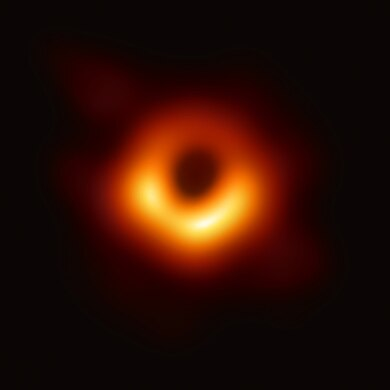
\includegraphics[width=4cm, height=4cm]{Pictures/bl}
    \caption{Direct radio image of a supermassive black hole at the core of Messier 87.}
    \label{fig:bl}
\end{figure}

\begin{center}    
Black holes are commonly classified according to their mass, independent of angular momentum, \textbf{$J$}. The size of a black hole, as determined by the radius of the event horizon, or \textit{Schwarzschild} radius, is proportional to the mass, \textbf{M}, through: 

$$r_s=\frac{2GM}{c^2} \approx 2.95 \frac{M}{M_s}km$$

where $r_s$ is the \textit{Schwarzschild} radius and $M_s$ is the mass of the \textbf{Sun}.\\
See table~\ref{tab:bl}
\end{center}

\newpage

\hrulefill

\textbf{Timeline of black hole physics:}
\begin{itemize}[label={--}]
  \item 1640 — Ismaël Bullialdus suggests an inverse-square gravitational force law
  \item 1676 — Ole Rømer demonstrates that light has a finite speed
  \item 1684 — Isaac Newton writes down his inverse-square law of universal gravitation
  \item 1758 — Rudjer Josip Boscovich develops his theory of forces, where gravity can be repulsive on small distances. So according to him strange classical bodies, such as white holes, can exist, which won't allow other bodies to reach their surfaces
  \item 1784 — John Michell discusses classical bodies which have escape velocities greater than the speed of light
  \item 1795 — Pierre Laplace discusses classical bodies which have escape velocities greater than the speed of light
\end{itemize}

\hrulefill

\textbf{List of most massive black holes:}
\begin{enumerate}
  \item Phoenix A
  \item 4C +74.13
  \item TON 618
  \item Holmberg 15A
  \item IC 1101
\end{enumerate}

\hrulefill

\textbf{Black hole classifications:}
\begin{table}[hb]
\centering
\begin{tabular}{||c | c | c |} 
 \hline
 Class & Approx. mass & Approx. radius \\ [0.5ex] 
 \hline\hline
 Ultramassive black hole & $10^9-10^{11} M_s$ & $>1,000AU$ \\ 
 \hline
 Supermassive black hole & $10^6-10^9 M_s$ & $0.001-400AU$ \\
 \hline
 Intermediate-mass black hole & $10^2-10^5 M_s$ & $10^3km\approx R_{Earth}$ \\
 \hline
 Stellar black hole & $2-150 M_s$ & $30 KM$ \\
 \hline
 Micro black hole & up to $M_{Moon}$ & up to $0.1mm$ \\
 \hline\hline
\end{tabular}
\label{tab:bl}
\caption{Black hole classifications.}
\end{table}